\documentclass{article}
\usepackage[letterpaper]{geometry}  
\usepackage{physics}
\usepackage[utf8]{inputenc}
\usepackage{sectsty}
\usepackage{amsmath,amssymb,amsthm}
\usepackage{titlesec}
\usepackage[titles]{tocloft}
\usepackage{tabularx}
\usepackage{graphicx}
\usepackage{float}
\usepackage{subcaption}
\usepackage{relsize}
\usepackage[final]{pdfpages}

\DeclareRobustCommand{\rchi}{{\mathpalette\irchi\relax}}
\newcommand{\irchi}[2]{\raisebox{\depth}{$#1\chi$}}

\newcommand{\HRule}{\rule{\linewidth}{0.5mm}} 
\allsectionsfont{\fontfamily{put}\mdseries\scshape}


\begin{document}
%\pagenumbering{gobble}
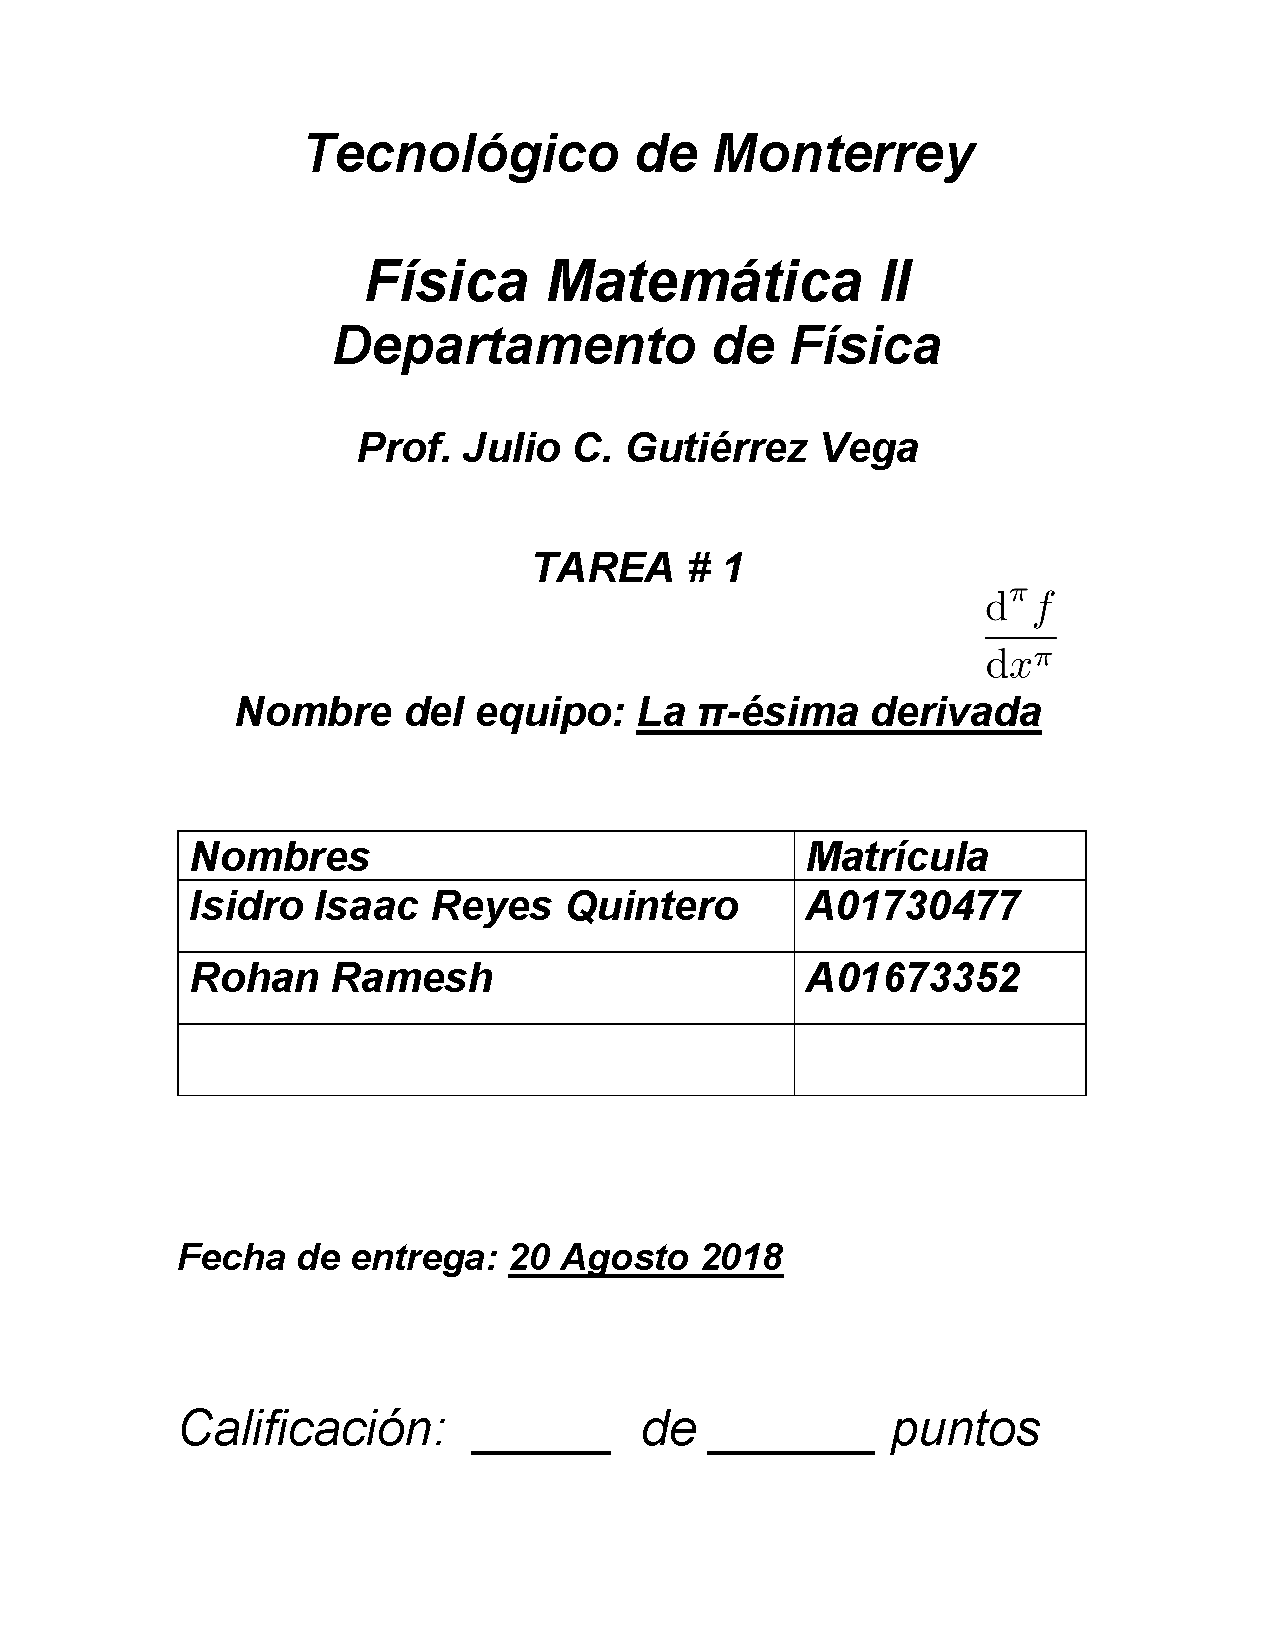
\includepdf{portada.pdf}
\section*{1)}
\begin{quote}
\textit{?`Bajo cuál condición tres puntos distintos $z_1$, $z_2$ y $z_3$ estarán sobre una misma recta?}
\end{quote}\hspace{0.5cm}\\
Consideramos los siguientes números complejos:
$$ z_{21}=z_2 - z_1=r_{21}e^{i\theta_{21}} \qquad z_{31}=z_3 - z_1=r_{31}e^{i\theta_{31}}$$
Para que los números queden sobre la misma recta, los ángulos de los números tienen que cumplir que $\theta_{21}=\pm \theta_{31}$. Esto nos permite escribir la condición de la siguiente manera:
$$\boxed{|\arg\left(z_2 - z_1\right)|=|\arg\left(z_3 - z_1\right)|}$$

\section*{2)}
\begin{quote}
\textit{?`Bajo cuál condición cuatro puntos distintos $z_1$, $z_2$, $z_3$ y $z_4$ estarán sobre una misma circunferencia?}
\end{quote}\hspace{0.5cm}\\
Consideramos que el punto $z_3$ es el punto más lejano de $z_1$, es decir, $|z_3-z_1|>|z_2-z_1|$ y $|z_3-z_1|>|z_4-z_1|$. Si no cumple con esto, se cambia el orden de los puntos de tal manera que sea cierto(si $z_2$, $z_3$ y $z_4$ son equidistantes a $z_1$, entonces los puntos no son sobre la misma circunferencia dado que $z_1$ sería el centro de un circulo único que pasa por los otros puntos).Ahora podemos utilizar el \textbf{teorema de Ptolemy} para definir la condición para que los 4 puntos queden sobre la misma circunferencia:
$$\boxed{|z_3-z_1||z_4-z_2|=|z_2-z_1||z_4-z_3|+|z_4-z_1||z_3-z_2| } $$

\section*{3)}
\begin{quote}
\textit{?`Bajo cuál condición n puntos distintos $z_1$, $z_2$, $z_3$, ..., $z_n$ estarán sobre una misma esfera tridimensional?}
\end{quote}\hspace{0.5cm}\\
Dado que todos los números complejos están definidos por 2 números reales(o dos grados de libertad) y sólo se requiere dos números reales para describir la superficie de una esfera, \textbf{todos los números complejos pertenecen a la misma esfera tridimensional}. Ej: \emph{Esfera de Riemann}.

\section*{4)}
\begin{quote}
\textit{Representar el conjunto de puntos
$$ \Re \left[(a + i)z + b\right]=0$$
con $a$, $b$ $\in$ $\mathbb{R}$ y explicar el significado geométrico de $a$ y $b$. }
\end{quote}\hspace{0.5cm}\\
Dado que $z=x+iy$, la expresión dada se puede escribir como:
$$\Re\left[ax - y+b +iay + ix)\right]= 0\qquad \Rightarrow\qquad ax-y+b=0 $$
Esto claramente es la ecuación de una línea recta, $a$ describe la pendiente de la línea y $b$ es la ordenada en el origen. A continuación se muestra una gráfica del conjunto de puntos, con valores $a$ y $b$ generados aleatoriamente. 
\begin{center}
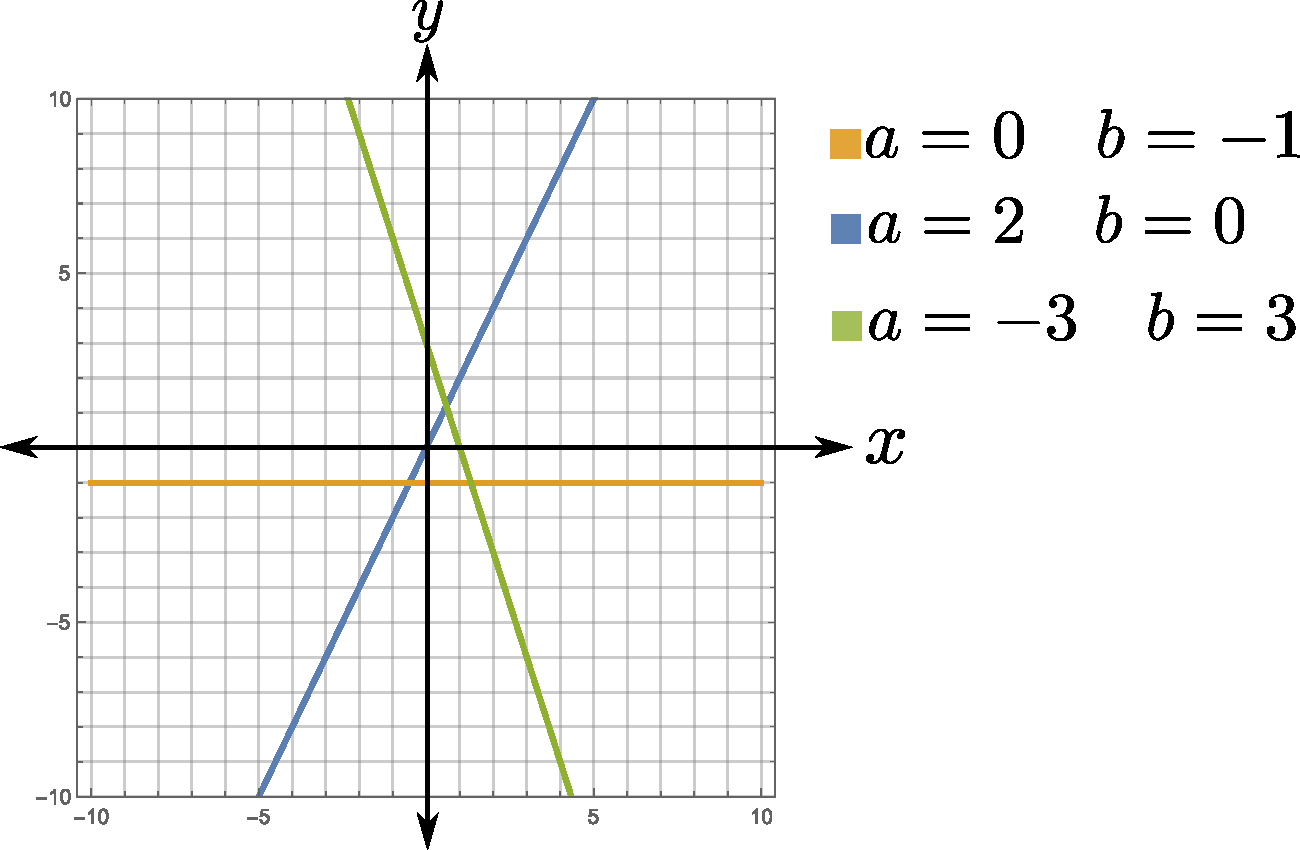
\includegraphics[scale=0.5]{fig1.pdf}
\end{center}


\section*{5)}
\begin{quote}
\textit{Dibuja en el plano complejo las regiones definidas por las siguientes relaciones }
\end{quote}\hspace{-1.5cm}\\
\subsection*{a) $|z-z_0|<R$}
La región representa todos los puntos en el plano complejo que se encuentran a una distancia menor a $R$ de $z_0$. En coordenadas cartesianas, la región está descrita por:
$$\sqrt{(x-x_0)^2 +(y-y_0)^2}<R $$
a continuación se muestra la región utilizando los siguientes valores:
$$z_0= 0.898998 + i 4.53115 \qquad R=4$$
\begin{center}
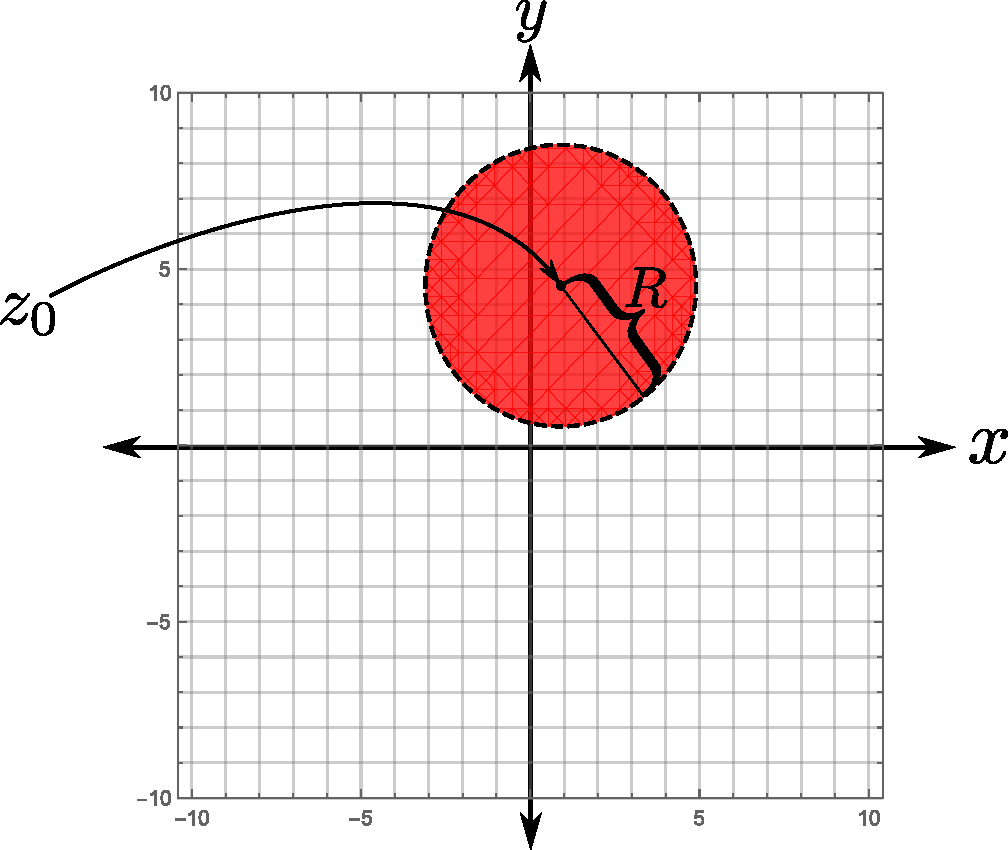
\includegraphics[scale=0.5]{fig2.pdf}
\end{center}







\subsection*{b) $\Re[z^2]=4$}
La expresión dada se puede simplificar a lo siguiente:
$$\Re[x^2-y^2+2ixy]=x^2-y^2=4 $$ 
Esto describe una hipérbola como se muestra en la siguiente gráfica:
\begin{center}
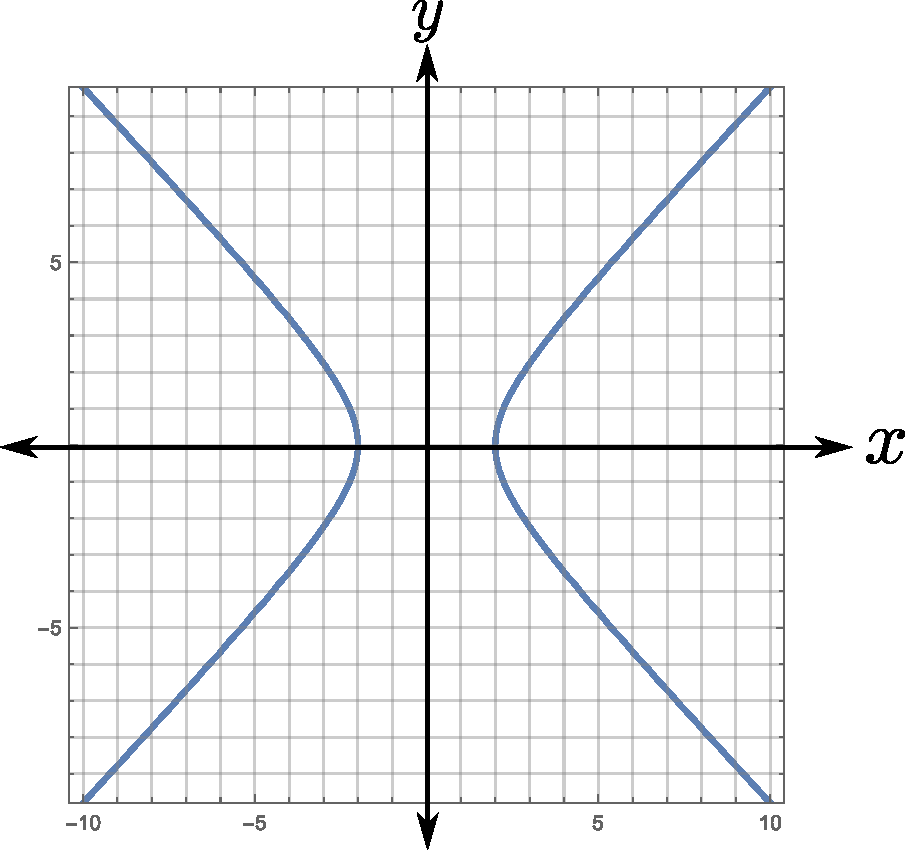
\includegraphics[scale=0.5]{fig3.pdf}
\end{center}


\subsection*{c) $\Re[e^{i\pi/2}z]=0$}
Simplificando, obtenemos:
$$\Re[ix-y]=-y=0 $$
\begin{center}
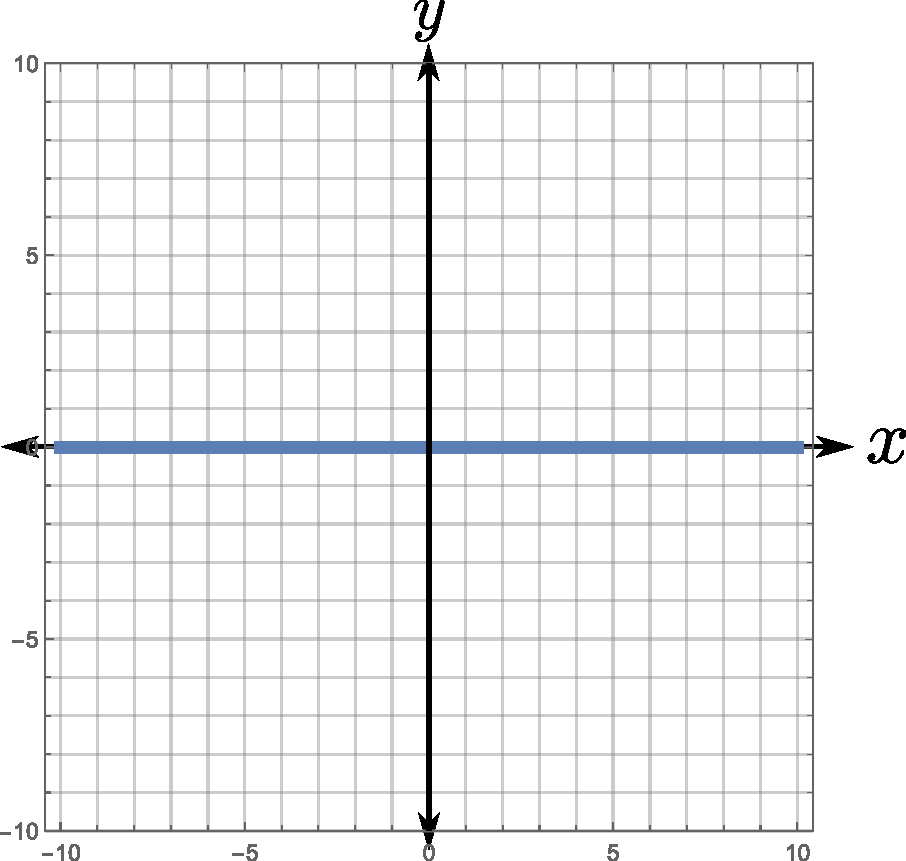
\includegraphics[scale=0.5]{fig4.pdf}
\end{center}

\subsection*{d)$|z-1+i|+|z+1-i|=6$}
Si consideramos que $z_0\equiv 1-i$, entonces podemos escribir la relación como:
$$|z-z_0|+|z+z_0|=6$$
Esto es la definición de un ellipse con focos en $z_0$ y $-z_0$. 
\begin{center}
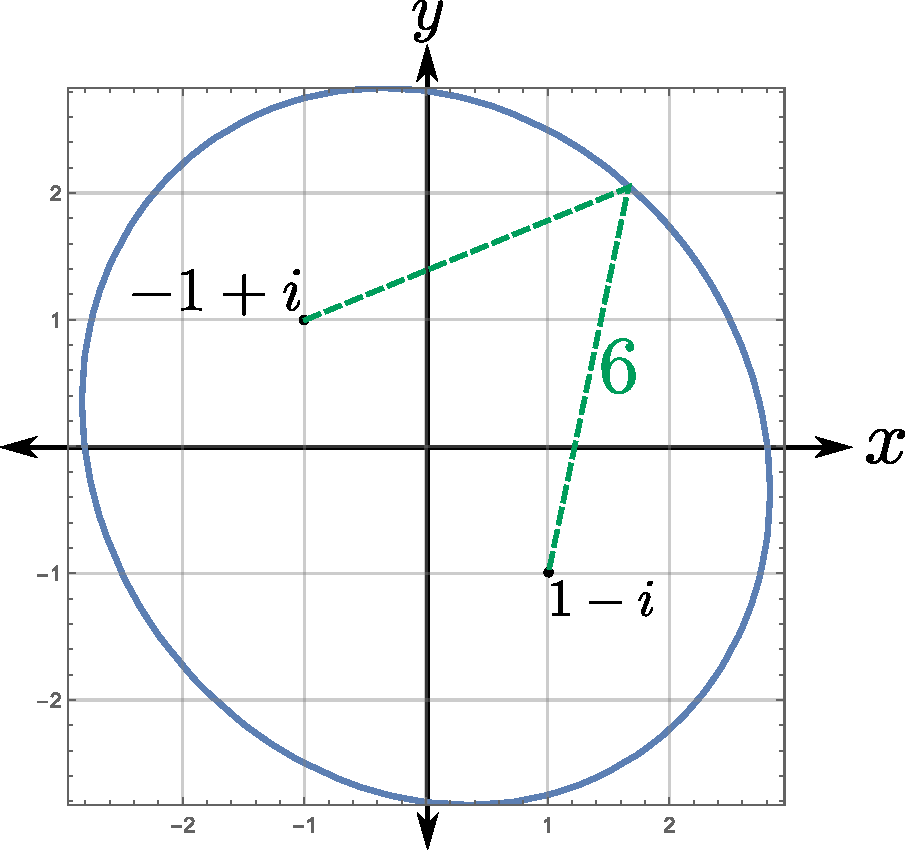
\includegraphics[scale=0.5]{fig5.pdf}
\end{center}

\subsection*{e)$\dfrac{e^{[\Im(z)]^2}}{e^{|z|^2}}-\Im(z)=0 $}
Simplificando, obtenemos:
$$\dfrac{e^{y^2}}{e^{x^2+y^2}}-y=0 \qquad\Leftarrow\qquad y=e^{-x^2}$$
la cual describe una campana gaussiana, como se muestre en al siguiente gráfica:
\begin{center}
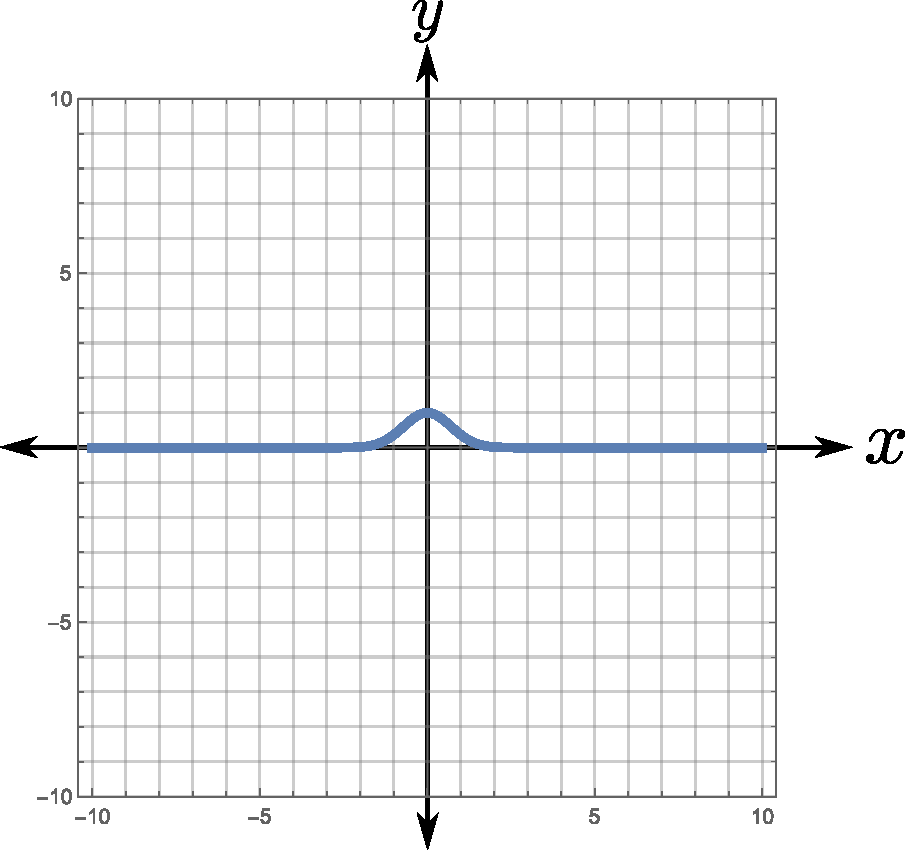
\includegraphics[scale=0.5]{fig6.pdf}
\end{center}

\section*{6)}
\begin{quote}
\textit{Encontrar y graficar cuidadosamente la región en el plano $w = u + iv$ que corresponde a la región triangular limitada por las rectas $x = 1$, $y = 1$ and $x+y = 1$ bajo la transformación $w = -z^2$}
\end{quote}\hspace{0.25cm}\\
Escribiendo explicitamente la transformación,obtenemos:
$$w=f(z)=-z^2=(y^2-x^2)+i(-2xy)$$
$$u=y^2-x^2 \qquad v=-2xy$$
utilizamos las siguientes parametrizaciones de las rectas dadas para generar las curvas correspondientes en el espacio $w$:
$$x=1 \quad y=t \qquad \rightarrow \qquad u=t^2-1 \quad v=-2t $$
$$x=t \quad y=1 \qquad \rightarrow \qquad u=1-t^2 \quad v=-2t $$
$$x=t \quad y=1-t \qquad \rightarrow \qquad u=2t-1 \quad v=2t(t-1) $$
utilizando estas curvas se generó la siguiente gráfica:
\begin{center}
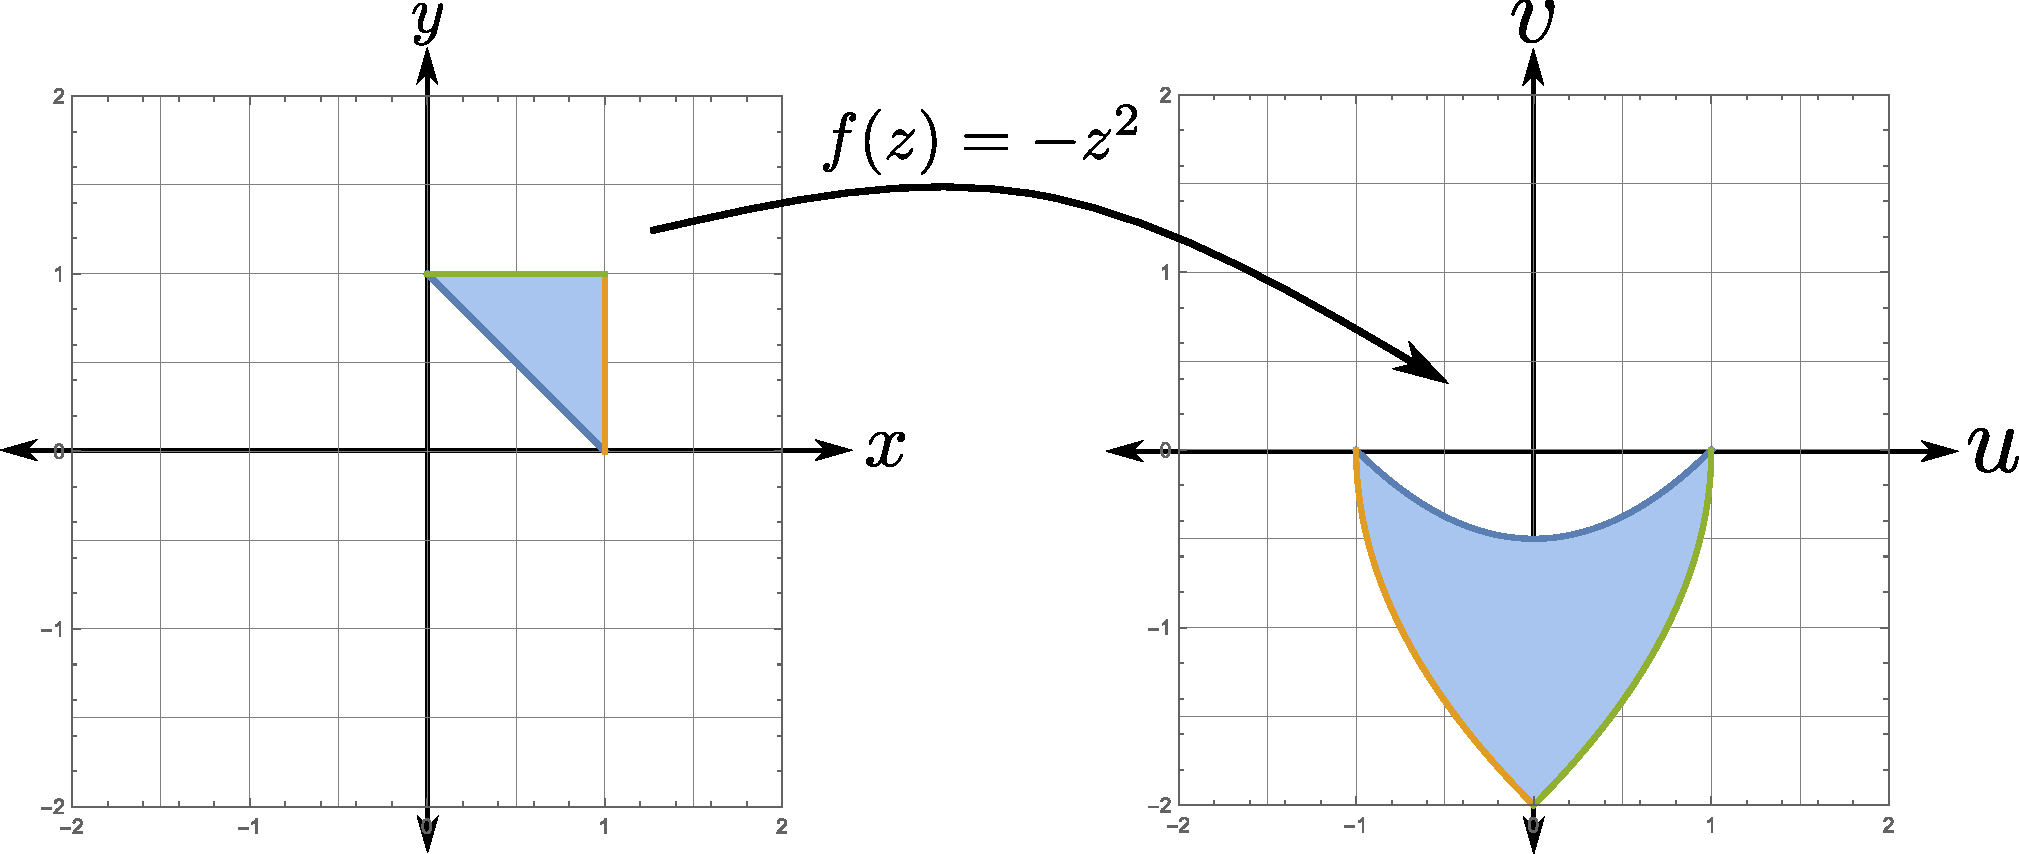
\includegraphics[scale=0.45]{fig7.pdf}
\end{center}

\section*{7)}
\begin{quote}
\textit{?`Cómo se transforman las líneas coordenadas del plano z cuando se aplica esta transformación?
$$e^z =\dfrac{a-w}{a+w}$$
donde $a$ es una constante compleja en general y $w = u + iv$. Para ilustrar sus conclusiones grafiquen cuidadosamente la imagen en el plano $w$ del rectángulo definido por los puntos $z_1 = 1 + i$, $z_2 = 3 + i$, $z_3 = 3 + 2i$ y $z_4 = 1+2i$.}
\end{quote}\hspace{0.25cm}\\
Queremos despegar la expresión para $w=f(z)$. Primero, tomamos el logaritmo de ambos lados:
$$z=\ln\dfrac{1-w/a}{1+w/a}$$
recordando que:
$$\tanh^{-1}(s)=\dfrac{1}{2}\ln\dfrac{1+s}{1-s}$$
podemos decir que:
$$z=2\tanh^{-1}\left(\dfrac{-w}{a}\right) \qquad \Rightarrow \qquad  w=-a\tanh\left(\dfrac{z}{2} \right)$$
Ya sabemos que el efecto del valor de $a$ escala y rota la transformación por las propiedades de los números complejos. Por lo tanto en las siguientes gráficas se utilizarán los valores:
$$a=1 \qquad a=e^{i\pi/4}\qquad a=2e^{i3\pi/2}$$
\begin{center}
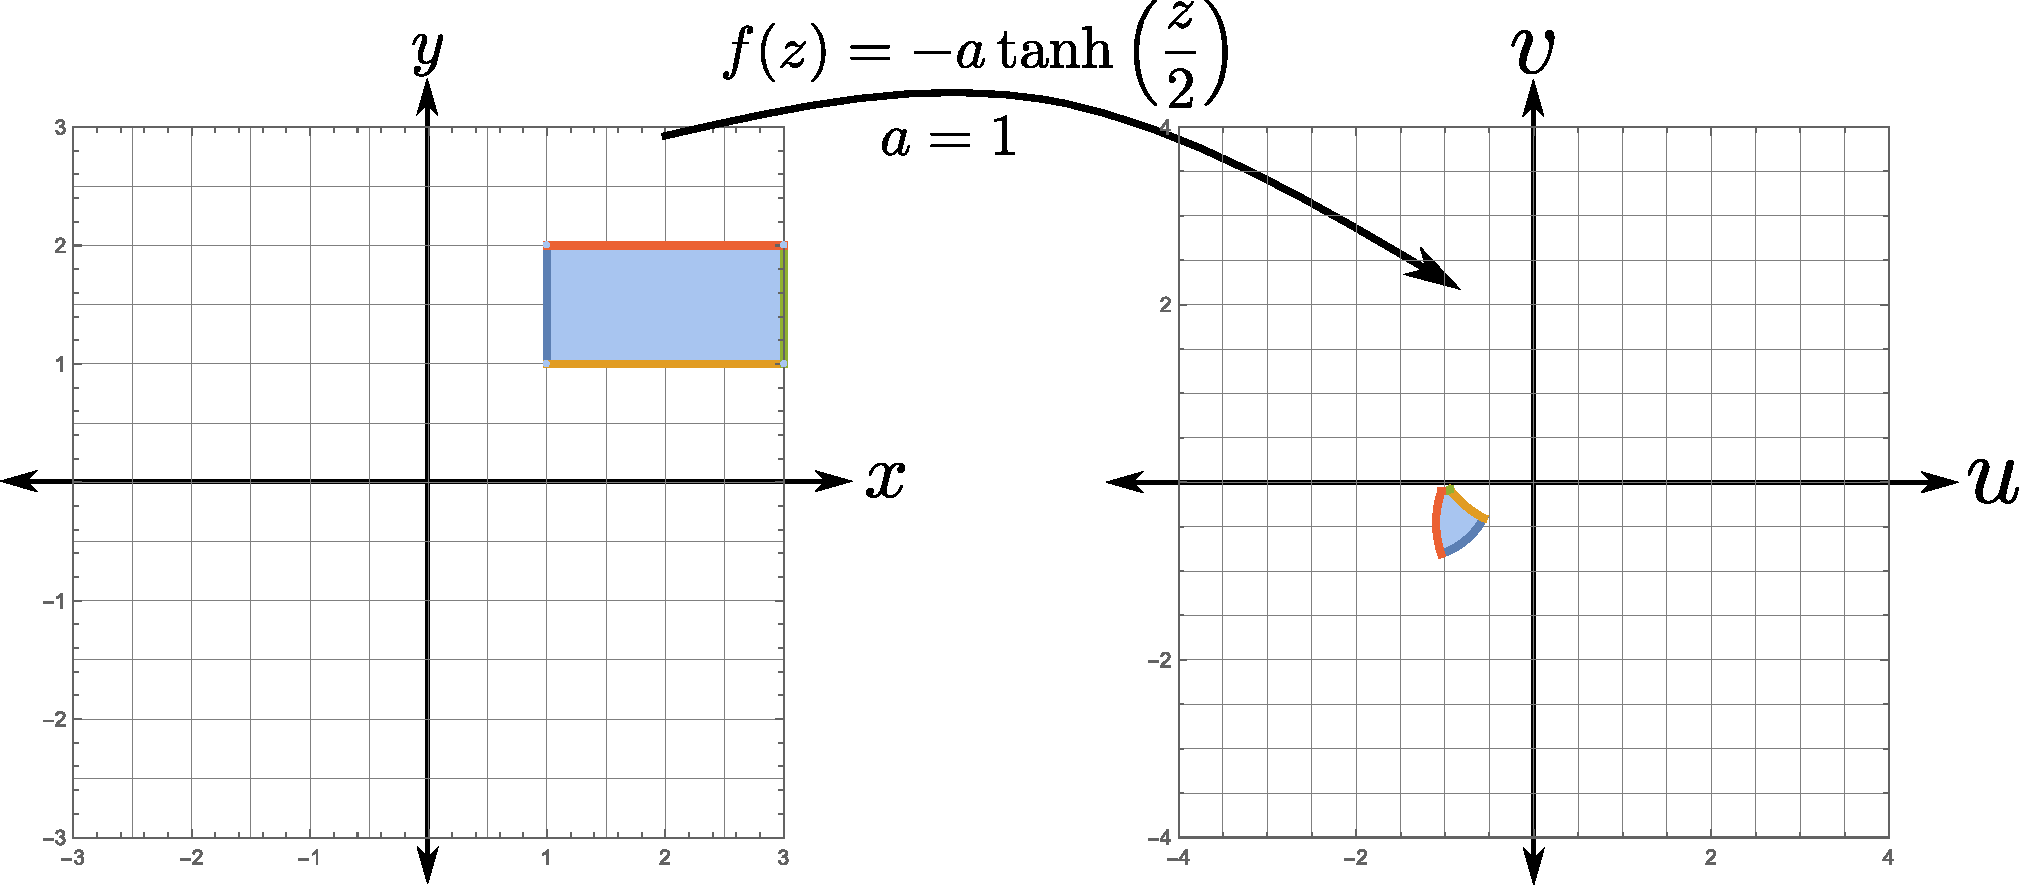
\includegraphics[scale=0.45]{fig8.pdf}
\end{center}
\begin{center}
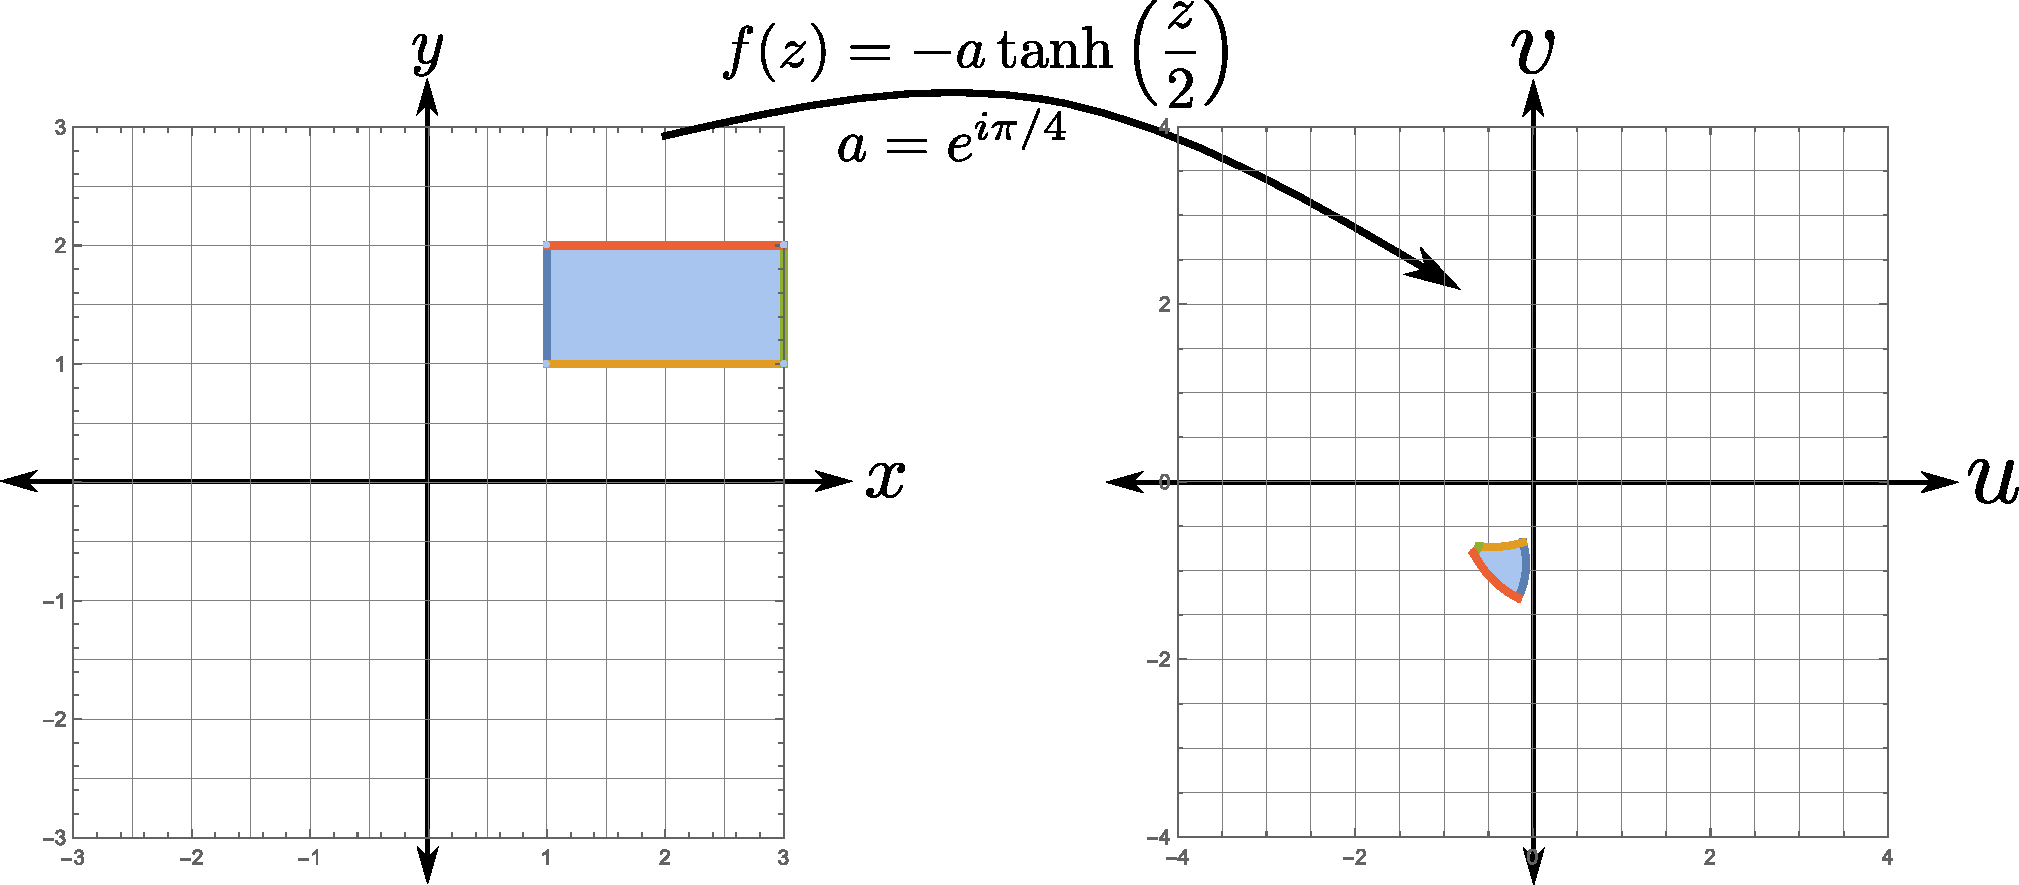
\includegraphics[scale=0.45]{fig9.pdf}
\end{center}
\begin{center}
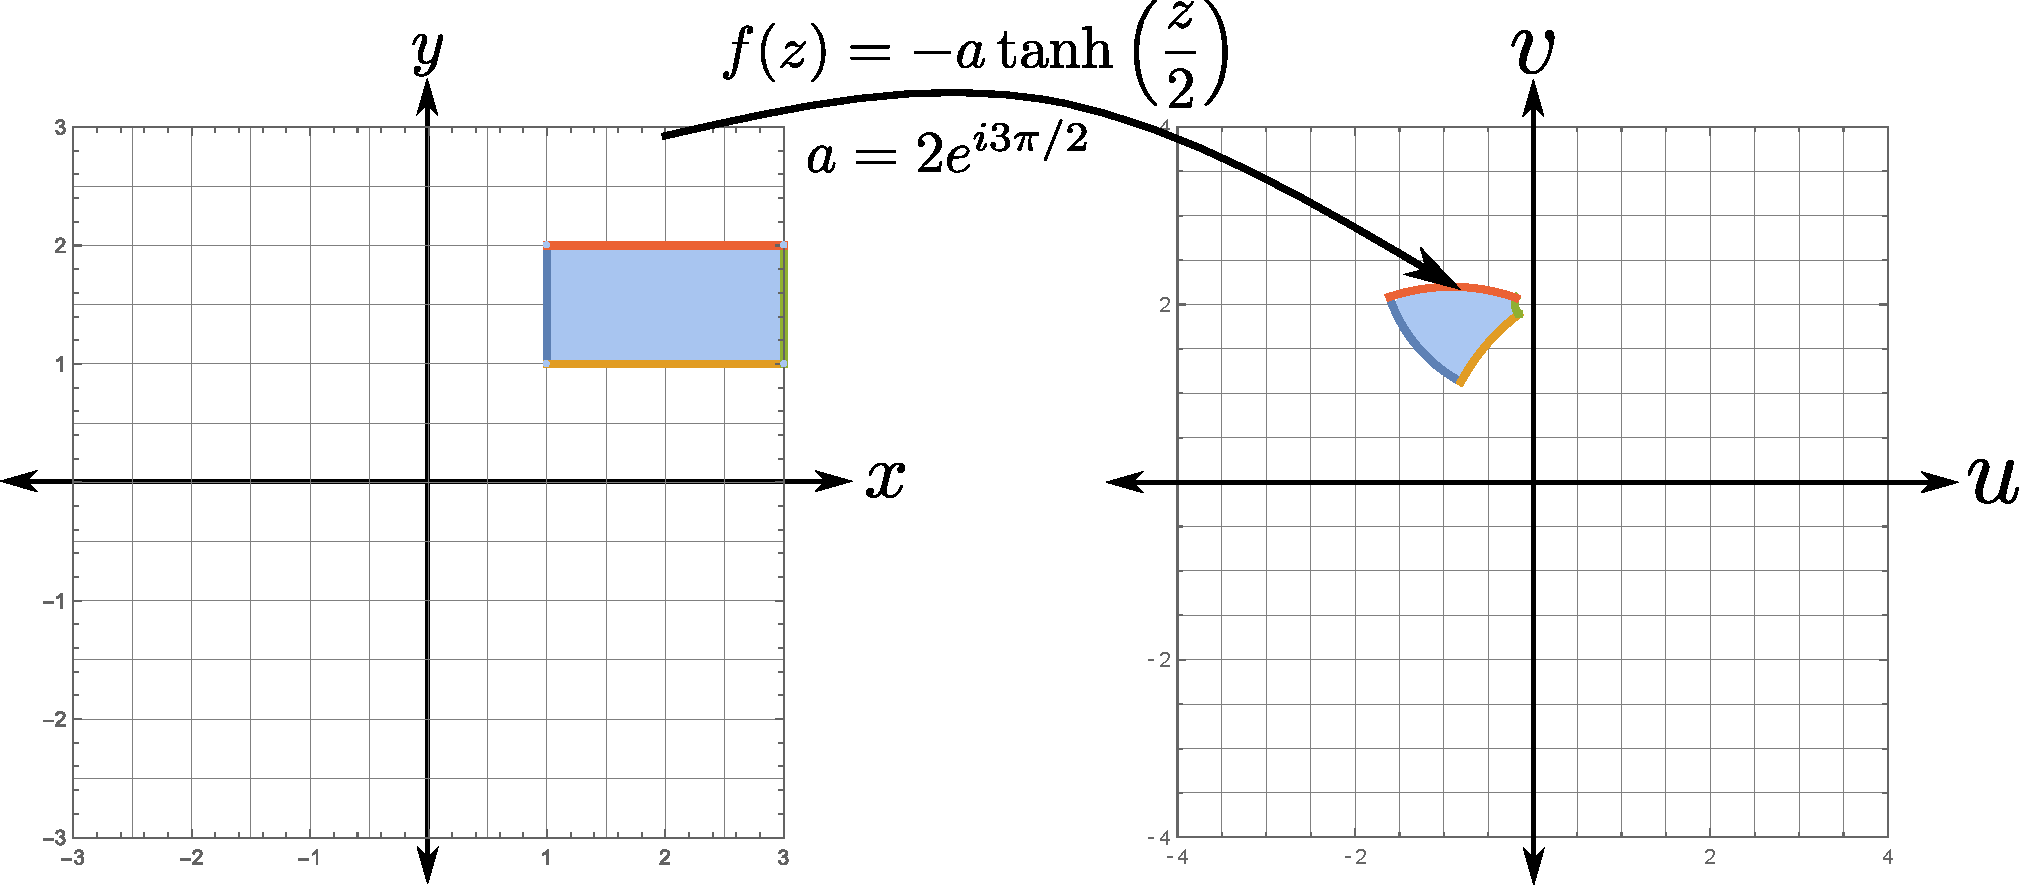
\includegraphics[scale=0.45]{fig10.pdf}
\end{center}

\end{document}